\documentclass{article}


% ready for submission
\usepackage{neurips_2025}



\usepackage[utf8]{inputenc} % allow utf-8 input
\usepackage[T1]{fontenc}    % use 8-bit T1 fonts
\usepackage{hyperref}       % hyperlinks
\usepackage{url}            % simple URL typesetting
\usepackage{booktabs}       % professional-quality tables
\usepackage{amsfonts}       % blackboard math symbols
\usepackage{nicefrac}       % compact symbols for 1/2, etc.
\usepackage{microtype}      % microtypography
\usepackage{xcolor}         % colors
\usepackage{graphicx}
\usepackage{amsmath}
\usepackage{algorithm}
\usepackage{algpseudocode}
\usepackage{caption}
\usepackage{svg}
\usepackage{tikz}
\usepackage{subcaption}
\usepackage{array}
\usepackage{tabularx}
\usepackage{threeparttable}
\usepackage{makecell} 
\usepackage{pdflscape}
\usepackage{float}
\usepackage{verbatim}
\usepackage{tocloft}  % 控制目录样式

\usepackage{bbm}

\setlength{\cftsecindent}{1.5em}
\setlength{\cftsubsecindent}{3em} 
\setlength{\cftsubsubsecindent}{4.5em}


\DeclareMathOperator*{\argmax}{arg\,max}
\DeclareMathOperator*{\argmin}{arg\,min}
\DeclareMathOperator*{\Hugeexpect}{\resizebox{12pt}{!}{$\mathbb{E}$}}
\DeclareMathOperator*{\expect}{\mathbb{E}}



\begin{document}

\begin{center}
    \LARGE \textbf{Supplementary Materials}
\end{center}

\vspace{1em}


\tableofcontents

\renewcommand{\thefigure}{S\arabic{figure}}
\setcounter{figure}{0}
\renewcommand{\thetable}{S\arabic{table}}
\setcounter{table}{0}

\appendix

\section{Human experimental details}
\label{sec: experiment}


\subsection{Participants} \label{sec: A.1}
Twenty-seven participants (15 females; age range: 18–25 years) were recruited for the experiment. Three participants voluntarily withdrew due to persistent difficulties with the learning task and were excluded from all subsequent analyses. All participants had normal or corrected-to-normal vision, reported no color vision deficiencies, and had no known history of psychiatric disorders. Written informed consent was obtained prior to participation, and monetary compensation was provided following the completion of the study.

\subsection{Stimuli} \label{sec: A.2}
To enable the generation of a virtually infinite set of stimuli within a four-dimensional continuous feature space, we developed a custom 2D line-drawing stimulus generation program, inspired by prior work~\cite{OLMAN2004227, NIPS2007_89d4402d}. Crucially, all stimuli were entirely novel, minimizing reliance on prior knowledge and providing a clean slate for learning. Each stimulus is composed of five parts: a fixed-length body (3.8° visual angle) and four parametrically varying features—head, neck, tail, and legs—whose lengths vary continuously from 0.25 to 1.25 times the body length. Each stimulus is rendered in either a left- or right-facing orientation. To eliminate any cues to 3D structure, all line angles were fixed, ensuring that morphological variation arises solely from differences in feature lengths.


\subsection{Procedure and design} \label{sec: A.3}
The experiment was conducted on a 27-inch LCD monitor with a resolution of 1920×1080 pixels and a refresh rate of 100 Hz. All stimuli were presented against a uniform gray background (RGB: 127, 127, 127). Experimental procedures were implemented using MATLAB (MathWorks Inc., Natick, MA, USA) in combination with Psychtoolbox-3. Participants used a headrest during tasks to minimize head movements and maintain a 60 cm viewing distance, ensuring a 3.8° visual angle for the stimulus body length. Behavioral responses were recorded via keyboard input, while verbal reports were collected using a professional-grade audio recorder. 

\subsubsection{Preparation task}
Prior to the main learning task, participants completed two preparatory tasks: a \textbf{free exploration task} (Fig. \ref{fig:S1}A), followed by a \textbf{perceptual calibration task} (Fig. \ref{fig:S1}B). 

The \textbf{free exploration task} was designed to familiarize participants with the length range of each feature dimension. In the task, participants manipulated an interactive stimulus by dragging morphological nodes (head, neck, tail, or legs) while the body remained fixed as a reference. Leg adjustments automatically synchronized the remaining three limbs to preserve quadrupedal symmetry. A flip button enabled left-right orientation changes. Task duration was limited to 5 minutes.

We employed a \textbf{perceptual calibration task} to estimate \textit{just-noticeable differences} (JNDs) along each feature dimension for individual participants. This involved a pairwise stimulus matching paradigm. On each trial, participants viewed two stimuli--a \textit{reference} stimulus and an \textit{adjustable} stimulus--displayed in either the same (e.g., left-left) or opposite orientations (e.g., left-right) to eliminate orientation-specific estimation bias. Each stimulus was created by randomly combining four features, with each feature dimension uniformly sampled at seven levels across its full range. Stimuli were vertically jittered on screen to prevent pixel-wise template matching. Using the same interactive interface as the free exploration task, participants adjusted the modifiable stimulus via mouse-drag to match the reference stimulus as closely as possible, regardless of vertical position or horizontal orientation. This design ensured responses reflected perceived feature differences rather than superficial pattern matching.

During the perceptual calibration, participants completed 192 trials covering all pairwise comparisons across the seven sampling levels for each feature. Mandatory rest periods (minimum 1 minute) were enforced after every 24 trials to prevent fatigue. For each feature, JND were estimated by calculating the distribution of discrepancies between \textit{final-adjusted} and \textit{reference} stimuli across all trials. The resulting means and standard deviations of these perceptual errors per feature parameterized individualized perceptual noise in subsequent computational modeling.

\begin{figure}[t]
    \centering
    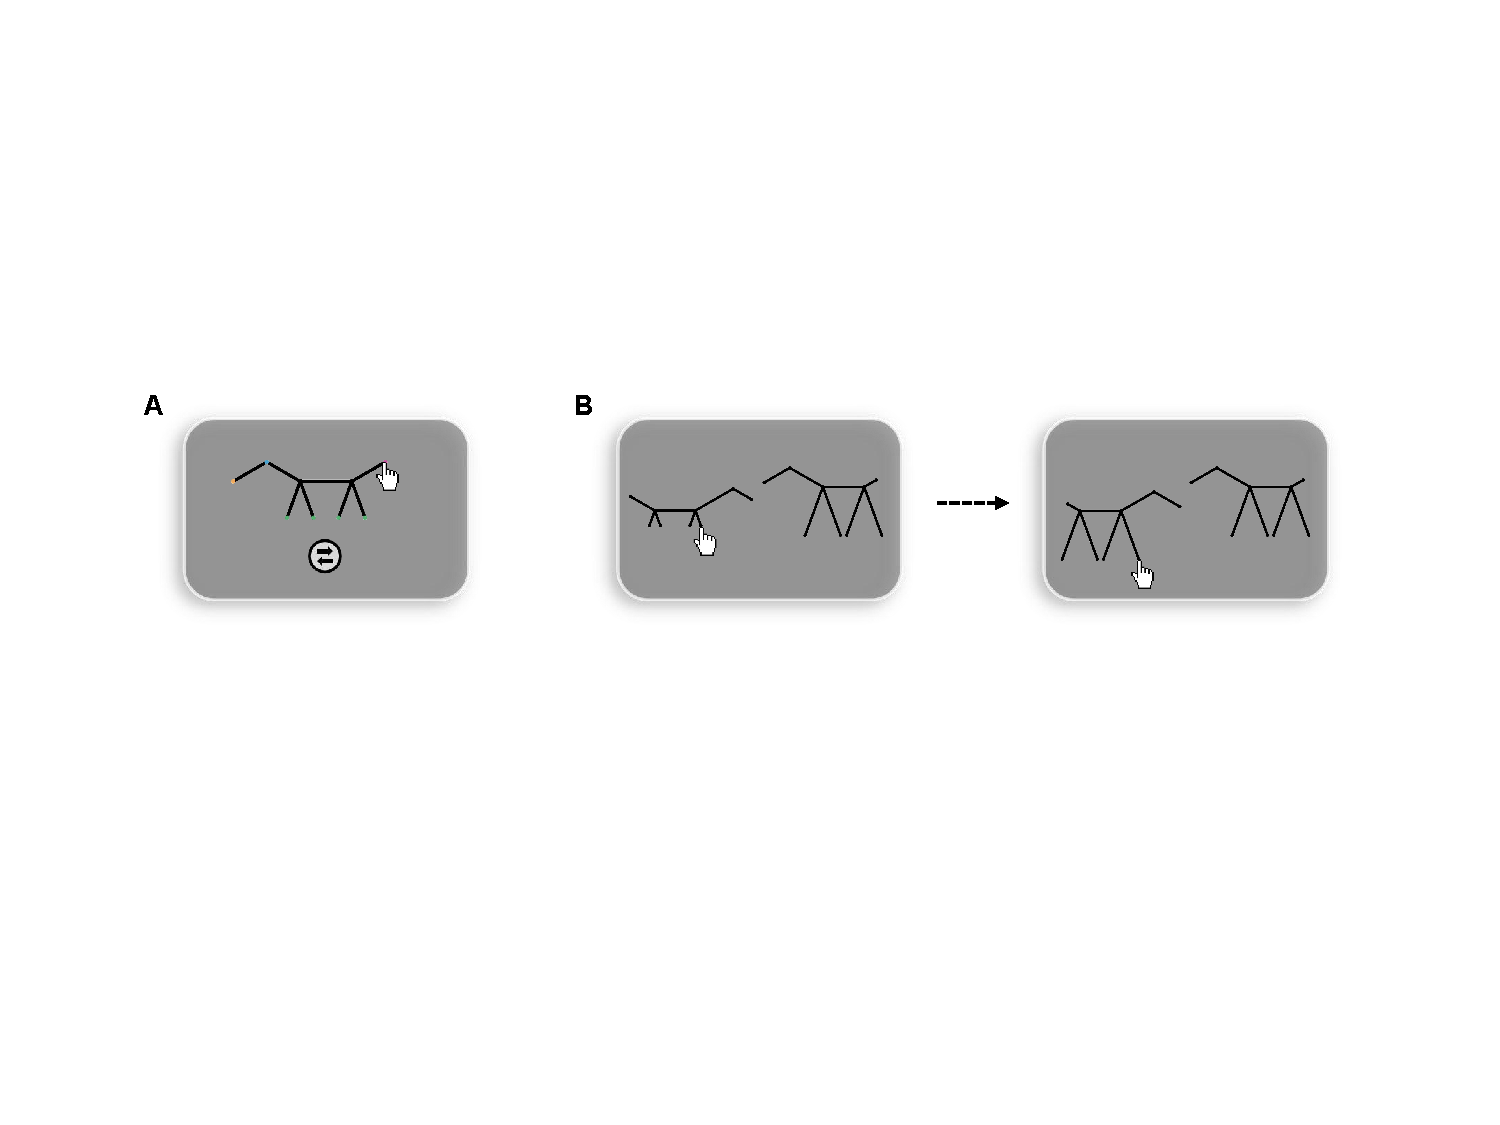
\includegraphics[width=1\textwidth, trim=2cm 8.3cm 2cm 6.6cm, clip]{figs/FigureS1.pdf}
    \caption{Preparation tasks. \textbf{(A)} Free exploration task: participants use the mouse to drag nodes or click the flip button to toggle the left–right orientation of each stimulus. \textbf{(B)} Perceptual calibration task: participants adjust the left stimulus to match the right stimulus as closely as possible in shape.}
    \label{fig:S1}
\end{figure}

\subsubsection{Learning task}
Participants were trained to categorize stimuli with infinite variations in dimensional feature space into a limited number of distinct groups. This design mirrors real-world challenges where learners must solve an ill-posed inverse problem: iteratively selecting and re-weighting relevant features from rich sensory inputs to derive low-dimensional categorical labels. 

Three different learning conditions were implemented using a between-subjects design. In \textbf{Task 1}, a simple two-category rule was based on a single randomly assigned feature, with the midpoint of the full range serving as the deterministic boundary between categories F and J (e.g., F = leg length > 0.5, J = leg length < 0.5, in a normalized range from 0 to 1). \textbf{Task 2} employed a four-category rule requiring integration of three features to form a hierarchical structure: four subordinate categories (F, G, H, J) nested under two basic-level categories (e.g., F\&H vs. J\&G), again using midpoint boundaries. For example, leg length (long vs. short) determined the basic-level categories, while combinations of neck and head lengths determined the four subordinate categories within each basic level. Feedback signals explicitly revealed the nested structure: 1 = correct at both levels, 0.5 = correct at basic level only, 0 = incorrect at both levels. \textbf{Task 3} used the same four-category structure but without hierarchical feedback—participants received binary feedback (1 = correct, 0 = incorrect) based solely on subordinate-level accuracy. Most of the participants in this condition reported not recognizing the hierarchy after successful learning. Crucially, participants received no information on what features or rules to use for categorization prior to training.

An adaptive learning procedure was implemented to avoid excessively long training sessions. Training blocks consisted of 64 trials each. We computed learning accuracy and \textit{d-prime} \footnote{The \textit{d-prime} ($d'$) score for each category was computed as $d' = Z(\text{hit rate}) - Z(\text{false alarm rate})$, where $Z(\cdot)$ denotes the inverse cumulative distribution function of the standard normal distribution.} for each category per block, excluding trials with ambiguous stimuli (any feature value within the 0.45–0.55 range). Based on calculated \textit{d-prime} values, stimulus distributions were adaptively adjusted for subsequent blocks: better-learned categories (higher \textit{d-prime}) appeared less frequently. This resulted in individualized, adaptive stimulus sequences for each participant. Training continued until participants achieved >90\% accuracy for all categories within a block or reached the 25-block limit. All participants except voluntary withdrawals successfully completed the task within these limits. To prevent fatigue, mandatory rest periods (minimum 1 minute) were enforced every 16 trials within each block. See Fig. \ref{fig:S2} for each individual's learning performance in Task 2 and Task 3, reflecting the similar variability in Task 1 as we reported in Fig. 1D.

\begin{figure}[htp!]
    \centering
    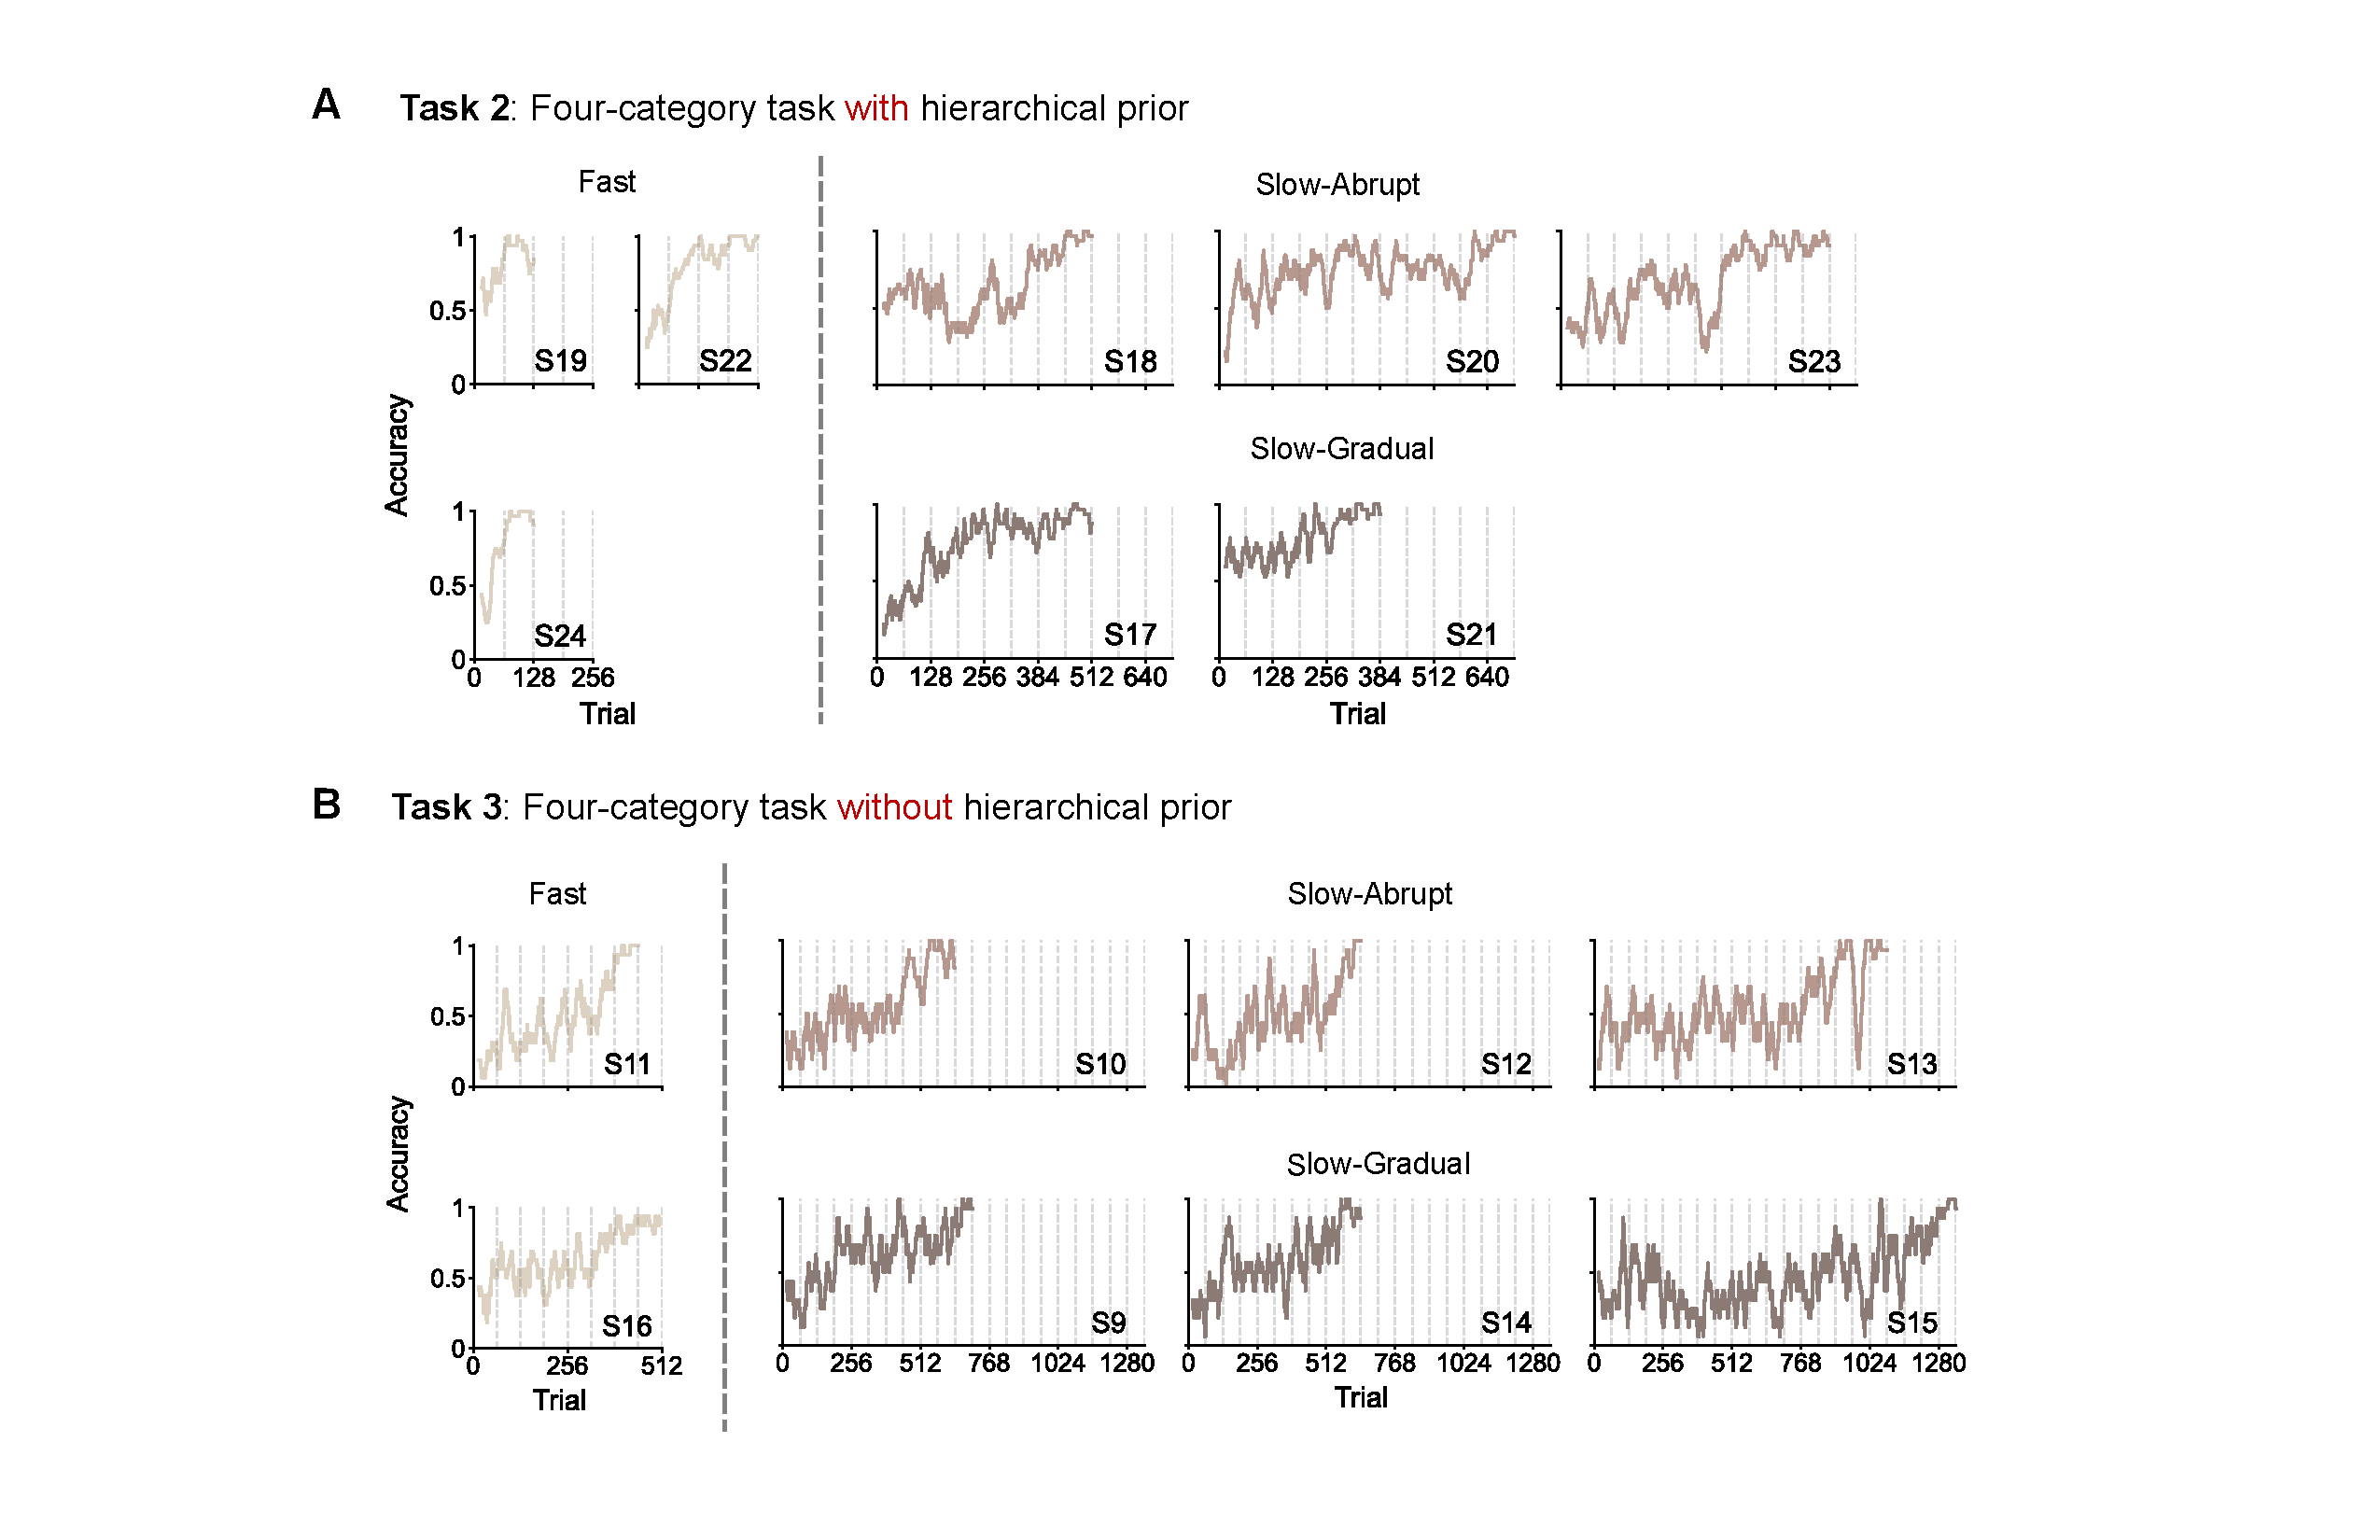
\includegraphics[width=1\textwidth, trim=5cm 1.5cm 5cm 1.5cm, clip]{figs/FigureS2.pdf}
    \caption{Learning performance in \textbf{(A)}Task 2  and \textbf{(B)}Task 3. Participants in each task could be broadly classified into three groups--fast (lightest brown), slower but abrupt (medium brown), and slower and gradual (darkest brown), as in Task 1.}
    \label{fig:S2}
\end{figure}


\subsection{Oral report coding} \label{sec: A.4}

In each learning trial, participants verbally reported the reasons for their category choice immediately after making a decision and prior to receiving feedback (with invalid or missing reports accounting for only 0.008\% of trials). We extracted structured internal representations from these verbal reports using a rule-based natural language parser that mapped spoken descriptions onto the four-dimensional feature space (see Table~\ref{tab:S1}). By concatenating these trial-wise representations, we reconstructed the learning trajectories shown in Fig. 1E of the main text.

Specifically, each report was first segmented into multiple expressions using commas as delimiters. For each expression, we identified and encoded the following components: (1) the description type (e.g., direct, comparative, superlative, exclusionary), (2) the referenced feature(s) (head, neck, tail, or legs), and (3) the described magnitude (e.g., “long,” “short,” “longer,” “longest”). Each expression was then translated into a numerical vector reflecting the inferred \textit{prototypical} values or weights associated with the mentioned features.  At the trial level, the final value for each feature was computed as the average of all values assigned to it across expressions; features not mentioned in any expression were assigned a default value of 0.5.


\begin{table}[htbp!]
\centering
\caption{Mapping rules from verbal reports to feature-space values}
\begin{tabularx}{\textwidth}{l X p{2.2cm} p{2cm}}
\toprule
\textbf{Description type} & \textbf{Example phrase (translated)} & \makecell[l]{\textbf{Mapped}\\ \textbf{feature(s)}} & \makecell[l]{\textbf{Prototypical}\\ \textbf{value(s)}} \\
\midrule
Direct & \makecell[l]{“The legs are long”\\ “The tail is short”\\ “The head is moderate”} & \makecell[l]{legs\\ tail\\ head} & \makecell[l]{0.75\\ 0.25\\ 0.5} \\
Comparitive & “The neck is longer than the head” & neck, head & \makecell[l]{neck = 2/3,\\ head = 1/3} \\
Overall & “All parts are short” & all features & 0.25 \\
Exclusive & “All parts are short except the tail” & all features & \makecell[l]{tail = 0.75,\\ others = 0.25} \\
Superlative & “The head is the longest” & all features & \makecell[l]{head = 0.8,\\ others = 0.4} \\

\bottomrule
\end{tabularx}
\label{tab:S1}
\end{table}

\section{Model details}
\label{sec: model}

\subsection{Geometrically regular partitions}

In our framework, categorization is geometrically formalized as partitioning the continuous feature space $\mathbf{X}$ into $N$ distinct regions, such that all stimuli within a region are assigned to the same category. 
Furthermore, motivated by both the structure of the original verbal report data and the need to ensure cognitive interpretability, we restrict the parametric partition $k\in\mathbf{X}^N$ to a finite set $\mathcal{K}$ of geometrically regular partitions (see Table \ref{tab:2} for the two-category partitions and Table \ref{tab:3} for the four-category partitions). Each partition $k\in\mathcal{K}$ must satisfy the following properties:

\textbf{(Symmetric)} Given that the $N$ categories are treated symmetrically, the partition regions must be invariant under permutations of the category labels. Specifically:

\begin{enumerate}
    \item The regions are isomorphic: they share identical shape and volume. Moreover, for any pair of regions, there exists a rigid transformation (i.e., rotation, translation, and reflection) that maps one onto the other.
    \item The center of $\mathbf{X}$ lies on the shared boundary of all regions.
\end{enumerate}

\textbf{(Connected)} Each category region in $\mathbf{X}$ is connected and star-shaped, hence simply connected.

\textbf{(Linear)} The boundary of each region is piecewise linear, composed of facets that lie within hyperplanes.

\textbf{(Non-isotropic)} We further prefer partitions whose boundaries align with salient geometric features of $\mathbf{X}$--for example, boundaries that coincide with its edges or intersect its vertices.

Based on the boundaries and regions defined by each partition, we further assume that participants represent each category using the geometric centroid of its corresponding region, effectively forming a \textit{Voronoi}-like partition. Each partition $k \in \mathcal{K}$ consists of $N$ \textit{Voronoi} centroids that serve as category prototypes. For any stimulus $\mathbf{x}$ in the feature space, its probability of belonging to each category $C_i$ is then computed as a softmax over the (negative) Euclidean distances to all category prototypes, modulated by an optimizable softness parameter $\beta$:
\begin{equation}
p(C_i | \mathbf{x},k) = \frac{e^{-\beta d(\mathbf{x},C_i|k)}}{\sum_{j=1}^{N} e^{-\beta d(\mathbf{x},C_j|k)}}. \tag{1}
\end{equation}

As a remark, the procedure of partition$\rightarrow$centroids$\rightarrow$centroid-determined \textit{Voronoi} partition
is NOT an identity map on partitions, even for those satisfying the above 4 properties. But the properties help the above procedure not be too far away from identity.

% \newpage
% \begin{landscape}
\begin{table}[H]
\centering
\begin{threeparttable}
\caption{Two-category partitions: Restricted partition types}
\begin{tabularx}{\textwidth}{X p{3cm} p{3.5cm} p{2.5cm}}
\toprule
\textbf{\# of dims. involved} & \textbf{Partition type} & \textbf{Boundary} & \textbf{\# of partitions} \\
\midrule
1 & \texttt{axis-aligned}\textsuperscript{*} & $x_i = 0.5$ & 4\\
2 & \texttt{equality} & $x_i = x_j$ & 6\\
2 & \texttt{sum} & $x_i + x_j = 1$ & 6 \\
4 & \texttt{mixed} & $x_i + x_j = x_k + x_l$  & 3\\
\bottomrule
\end{tabularx}
\begin{tablenotes}[para,flushleft]
\footnotesize
\textsuperscript{*} Indicates the ground-truth partition type used in the task design.\\
\textit{Note:} $i$, $j$, $k$, and $l$ denote distinct feature dimensions.
\end{tablenotes}
\label{tab:2}
\end{threeparttable}
\end{table}


\begin{table}[H]
\centering
\begin{threeparttable}
\caption{Four-category partitions: Restricted partition types}
\begin{tabularx}{\textwidth}{l l l l}
\toprule
\makecell[l]{\textbf{\# of dims.}\\ \textbf{involved}}
 & \textbf{Partition type} & \textbf{Boundaries} & 
 \makecell[l]{\textbf{\# of}\\\textbf{partitions}} \\
\midrule
2 & \texttt{axis-aligned * 2} & \makecell[l]{$\text{(1) } x_i = 0.5$,\\ $\text{(2) } x_j = 0.5.$} & 6\\
2 & \texttt{equality + sum} & \makecell[l]{$\text{(1) } x_i = x_j$,\\ $\text{(2) } x_i + x_j = 1.$} & 6\\
3 & \texttt{axis-aligned + equality} & \makecell[l]{$\text{(1) } x_i = 0.5$,\\ $\text{(2) } x_j = x_k.$} & 12\\
3 & \texttt{axis-aligned + sum} & \makecell[l]{$\text{(1) } x_i = 0.5$,\\ $\text{(2) } x_j + x_k = 1.$} & 12\\
4 & \texttt{equality * 2} & \makecell[l]{$\text{(1) } x_i = x_j$,\\ $\text{(2) } x_k = x_l.$} & 3\\
4 & \texttt{sum * 2} & \makecell[l]{$\text{(1) } x_i + x_j = 1$, \\ $ \text{(2) } x_k + x_l = 1.$} & 3\\
3 & \texttt{axis-aligned * 3}\textsuperscript{*} & \makecell[l]{$\text{(1) } x_i = 0.5$,\\ $\text{(2) } x_j = 0.5$ and $x_i < 0.5$,\\ $\text{(3) } x_k = 0.5$ and $x_i \geq 0.5.$} & 24\\
3 & \texttt{axis-aligned + equality + sum} & \makecell[l]{$\text{(1) } x_i = 0.5$,\\ $\text{(2) } x_j = x_k$ and $x_i < 0.5$,\\ $\text{(3) } x_j + x_k = 1$ and $x_i \geq 0.5.$} & 24\\
4 & \texttt{equality + axis-aligned * 2} & \makecell[l]{$\text{(1) } x_i = x_j$,\\ $\text{(2) } x_k = 0.5$ and $x_i < x_j$,\\ $\text{(3) } x_l = 0.5$ and $x_i \geq x_j.$} & 12\\
4 & \texttt{sum + axis-aligned * 2} & \makecell[l]{$\text{(1) } x_i + x_j = 1$,\\ $\text{(2) } x_k = 0.5$ and $x_i + x_j < 1$,\\ $\text{(3) } x_l = 0.5$ and $x_i + x_j \geq 1.$} & 12\\
4 & \texttt{Superlative} & $\{x_i = x_j\}$ for all $i \neq j$ & 2\\

\bottomrule
\end{tabularx}
\begin{tablenotes}[para,flushleft]
\footnotesize
\textsuperscript{*} Indicates the ground-truth partition type used in the task design.\\
\textit{Note:} $i$, $j$, $k$, and $l$ denote distinct feature dimensions.
\end{tablenotes}
\label{tab:3}
\end{threeparttable}
\end{table}
% \end{landscape}
% \newpage



\subsection{Hypothesis generator module} 

The hypothesis generator, as a core module, is implemented using pre-defined sampling strategies and a dynamically adjusted hypothesis set size to balance exploration and computational efficiency.

Specifically, we define three strategies for hypothesis selection: \textit{posterior-based exploitation} ($S_1$), \textit{cue-driven associative recall} ($S_2$), and \textit{stochastic exploration} ($S_3$). At every trial $t$ the learner firstly decides the amount of hypotheses to draw from each strategy, $(m_1^{(t)}, m_2^{(t)}, m_3^{(t)})$, then generates the next working hypothesis set $\mathcal H_{t+1}=\bigcup_{i=1}^3S_i^{(t)}$ from
\addtocounter{equation}{1}
\begin{eqnarray}
    S_1^{(t)} &\in&\left\{(\text{Top-}m_1^{(t)})(q_t(k);\mathcal{H}_{t}),\quad \text{No-Rep}(\pi(q_t(k)); m_1^{(t)})\right\}\\
   S_2^{(t)} &\in&\left\{(\text{Top-}m_2^{(t)})(s_t(k|\mathbf{x}_{t+1});\mathcal{K}\backslash{S_1^{(t)}}),\quad \text{No-Rep}(\pi(s_t(k|\mathbf{x}_{t+1})); m_2^{(t)})\right\}\\
   S_3^{(t)} &\sim&\text{Uniform}\!\left(\mathcal K\setminus(S_1^{(t)}\cup S_2^{(t)}),\;m_3^{(t)}\right) 
\end{eqnarray}
where $q_t(k)$ is the current posterior,  $s_t(k|\mathbf{x}_{t+1})$ denotes the associative similarity between the next stimulus $\mathbf x_{t+1}$ and partition $k$, and $\pi(\cdot)$ denotes a probabilistic transformation over input scores, mapping them into a distribution suitable for stochastic sampling without replacement.


\paragraph{Posterior-based exploitation.} As participants tend to exhibit a general consistency in their learning behavior, we incorporate an exploitation strategy $S_1$ based on the posterior over the hypothesis set from the previous trial, i.e., $S_1^{(t)}\subset{H_{t}}$. The posterior encodes information about the basic correctness of each hypothesis, serving as a principled guide for selecting promising candidates in the next trial. This selection process involves first determining the number of hypotheses to retain, $m_1^{(t)}$, followed by either selecting the top-$k$ based on posterior scores or sampling from the posterior distribution.


\paragraph{Cue-driven associative recall.} In this strategy, we assume that upon observing the next stimulus $\mathbf x_{t+1}$, participants may engage in associative recall, retrieving hypotheses whose category centroids closely resemble the stimulus, as if the stimulus serves as a cue that reactivates relevant prior structure. This process occurs before participants make the observable choice $c_{t+1}$, and can therefore be considered part of their internal inference during trial $t$.

Practically, the agent applies the current most probable hypothesis $h = \arg\max_{k'} p_{\text{post}}^{(t)}(k')$ to the new stimulus $\mathbf{x}_{t+1}$ and identifies the most relevant Voronoi centroid $\hat{j}$ in $h$ as:
\begin{equation}
\hat{j} := \arg\min_{j} \, d\left( \mathbf{x}_{t+1}, h_j \right), \tag{5}
\end{equation}
where $d(\cdot, \cdot)$ denotes the Euclidean distance in feature space.
Then, It selects (or samples) a subset of $m_2^{(t)}$ available hypotheses according to a similarity function $s_t(k \mid \mathbf{x}_{t+1})$, which measures the proximity between $h_{\hat{j}}$ and the centroids of the candidate hypothesis $k\in \mathcal{K}$:
\begin{equation}
s_t(k \mid \mathbf{x}_{t+1}) = \min_{i < N} \, d(h_{\hat{j}}, k_i). \tag{6}
\end{equation}


\paragraph{Stochastic exploration.} 
To model exploratory behavior, we introduce a stochastic mechanism that selects $m_3^{(t)}$ hypotheses uniformly at random from the hypothesis space 
$\mathcal{K}$, independent of past inference or current observations.

Notably, the above three strategies for $S_1$, $S_2$, and $S_3$ are executed sequentially to ensure that the resulting sets are disjoint.

\paragraph{Balancing exploration and exploitation.}
By rebalancing the amounts of hypotheses assigned to $S_1$, $S_2$, and $S_3$, the model dynamically controls the trade-off between exploitation and exploration. The general principle we follow is that stronger and more confident conclusions favor exploitation, while greater uncertainty calls for increased exploration. In practice, our model uses the \textit{entropy} of the posterior distribution as a measure of concludedness to adaptively adjust the proportion of hypotheses dedicated to each strategy, since the posteriors concentrated on one or two hypotheses (representing the state of being confident) have lower entropy and posteriors closer to uniform distribution have higher entropy.

\subsection{Optimization algorithms}

We illustrate the optimization procedure below using the full model (PMH-model), which integrates all three modules: perception, memory, and hypothesis generator. The same procedure is applied to all reduced model variants, with the corresponding cognitive module(s) omitted during optimization.

For each participant, we first perform a grid search over the memory parameters $(\gamma, w_0)$ to identify the setting that best accounts for their observed behavior. Specifically, for each candidate pair $(\gamma, w_0)$ in the discretized grid $(\Gamma^\sharp, W_0^\sharp)$, we apply Algorithm~\ref{alg:1} multiple times to simulate the learning process under a simplified base model $PM_0H_0$. Each simulation produces a sequence of predicted choices ${(\hat{c_t})_{t=1}^T}$ and posterior distributions $\left\{p_{post}^{(t)}(k)\right\}_{t=1}^T$ over hypotheses. For each simulated trajectory, we evaluate how closely the expected model-predicted performance (i.e., $\sum_t \mathbb{E}_{k\sim p_{\text{post}}^{(t)}}[p(c_t^\ast \mid \mathbf{x}_t, k)]$) matches the participant’s actual feedback trajectory $(r_t)_{t=1}^T$. The error-minimizing parameter pair $(\gamma^\ast, w_0^\ast)$ is selected as optimal. Using this optimal pair, we then simulate 1000 behavioral trajectories with the full $PMH$ model (Algorithm~\ref{alg:2}). Among these, the trajectory whose predicted performance best aligns with the observed behavioral profile is selected as the representative simulation for that participant. Here, Algorithm~\ref{alg:1} defines the generative process of learning under fixed memory parameters, while Algorithm~\ref{alg:2} wraps this procedure into a model selection and trajectory matching pipeline across the entire parameter grid.

\begin{algorithm}[htp]
\caption{$PM_0H_0$ Model as a Random Variable-valued Function}\label{alg:1}
\begin{algorithmic}[1]
\Statex \textbf{Input:} $\left\{(\mathbf x_t,c_t,r_t)\right\}_{t=1}^{T},\mathcal{H},\gamma,w_0$, $\sigma:X\rightarrow \mathbb{R}^N$ the error standard deviation
\Statex \textbf{Output:} ${(\hat{c_t})_{t=1}^T}, \left\{p_{post}^{(t)}(k)\right\}_{t=1}^T$
\Statex \textbf{Initialize:} $p_{post}^{(0)}(k) = \frac{1}{\left |\mathcal{H} \right |}$
\For{$t\gets1$ to $T_{max}$}
    \State $\boldsymbol{\varepsilon} \sim \mathcal{N}(\boldsymbol{\mu}, \boldsymbol{\Sigma})$\rule{0pt}{13pt}
    \State $\hat{\mathbf x} \gets \mathbf x + \boldsymbol\varepsilon$\rule{0pt}{13pt}
    \State $p_{post}^{(t)}(k)\gets BayesianWithMemory(p_{post}^{(t-1)}(k),\mathcal{H},\gamma,w_0)$\rule{0pt}{13pt}
    \State $\hat{(c)}_{t} \sim \mathbb{E}_{p_{\text{post}}^{(t)}(k)} \left( p(C \mid \hat{\mathbf x}, k) \right)$\rule{0pt}{13pt}
    \State $\mathcal{H} \gets$ $\mathcal{H_{\text{new}}}=S_1^{(t)}\cup S_2^{(t)}\cup S_3^{(t)}$\rule{0pt}{13pt}
\EndFor
\end{algorithmic}
\end{algorithm}



\begin{algorithm}[htp!]
\caption{$PMH$ Model}\label{alg:2}
\begin{algorithmic}[1]
\Statex \textbf{Input:} $\left\{(\mathbf x_t,c_t,r_t)\right\}_{t=1}^{T}$, $\mathcal{H},\gamma,w_0$, $(c_t^\ast)_{t=1}^T$ the correct class labels of data, $(\Gamma^\sharp, W_0^\sharp)$ discretization of $(\Gamma, W_0)$
\Statex \textbf{Output:} ${(\hat{c_t})_{t=1}^T}, \left\{p_{post}^{(t)}\right\}_{t=1}^T$
\Statex \textbf{Initialize:} $p_{post}^{(0)}(k) = \frac{1}{\left |\mathcal{H}_0 \right |},\mathcal{H}_0 $
\For{each $(\gamma^i, w_0^i) \in \Gamma^\sharp \times W_0^\sharp$}
    \For{$j \gets 1$ to $5$ (monte-carlo of size 5)}
        \State $\{^{{j}}\!c_t\}_{t=1}^T,\{^{{j}}\!p^{(t)}_{post}\}_{t=1}^T\sim PM_0H_0(\left\{(\mathbf x_t,c_t,r_t)\right\}_{t=1}^T, \mathcal{H}, \gamma,w_0)$
%         \State $e^{i,j} \gets error(\left\{(\mathbf x_t,c_t,r_t)\right\}_{t=1}^{T},\mathcal{H}_0,\gamma^{i,j},w_0^{i,j})$
    \EndFor
        \State $E(\gamma,w_0)\gets\min\limits_{j\in\{1,...,5\}}\left|\sum\limits_{t=1}^T{\expect\limits
        _{k\sim^{j}\!p_{post}^t}p(c^\ast_t|\mathbf x_t,k)}-\sum\limits_{t=1}^Tr_t\right|$
%     \State $e^i \gets \sum_{j=1}^{5} e^{i,j}$
%     \State $\gamma^*,w_0^* \gets \arg\min_{\gamma,w_0}e^i$    
\EndFor
\State $\gamma^\ast, w_0^\ast \gets \argmin\limits_{(\gamma,w_0)\in\Gamma^\sharp\times W_0^\sharp} E(\gamma,w_0)$
% \State $\gamma^\ast, w_0^\ast = \argmin\limits_{(\gamma,w_0)\in\Gamma\times W_0}
% \left\{\expect\limits_{\{C_t\}_{t=1}^T,P\sim PH_0M_0(\left\{(\mathbf x_t,c_t,r_t)\right\}_{t=1}^T, \mathcal{H}, \gamma,w_0)}\left|\sum\limits_{i=1}^T{\mathbbm{1}(C_t, c^\ast_t)}-\sum\limits_{i=1}^T{r_t}\right|\right\}$
\For{$\alpha \gets1$ to $1000$}\rule{0pt}{13pt}
    \State $(\{^\alpha\!c_t\}, \{^\alpha\!p_{post}^{(t)}\})  \sim PM_0H_0(\left\{(\mathbf x_t,c_t,r_t)\right\}_{t=1}^{T},\mathcal{H}_0,\gamma^*,w_0^*)$
\EndFor


\State $\left ( \hat{c},p_{post}  \right)_{best} \gets \argmin\limits_{\{^\alpha\!c_t\} ,\{^\alpha\!p_{post}^{(t)}\} }
\left|\sum\limits_{t=1}^T{\expect\limits
        _{k\sim^{\alpha}\!p_{post}^{(t)}}p(c^\ast_t|\mathbf x_t,k)}-\sum\limits_{i=1}^Tr_t\right|
$
\Statex \textbf{Return: } $ \left ( \hat{c},p_{post}  \right)_{best} $
\end{algorithmic}
\end{algorithm}









% \begin{algorithm}[htp]
% \caption{Compute $error$}
% \begin{algorithmic}[1]
% \Statex \textbf{Input:}  $\left\{(\mathbf x_t,c_t,r_t)\right\}_{t=1}^{T},\mathcal{H},\gamma,w_0$
% \Statex \textbf{Output:} $error$
% \State $ {(\hat{c_t})_{t=1}^T}, \left\{p_{post}^{(t)}(k)\right\}_{t=1}^T   \gets PH_0M_0(\left\{(\mathbf x_t,c_t,r_t)\right\}_{t=1}^{T},\mathcal{H},\gamma,w_0 )$
% \State $acc_{true}^t \gets \mathbb{I}[r_t = 1], \quad t = 1, \dots, T$
% \State $ acc_{pred}^t \gets \sum_{k} p_{post}^{(t)}(k) \cdot p_{true}^{(t)}(k), \quad t = 1, \dots, T$
% \State $error \gets \sum_{t=1}^{T} \left |  acc_{pred}^t - acc_{true}^t  \right | $
% \Statex \textbf{Return: } $ error$
% \end{algorithmic}
% \end{algorithm}


% \begin{algorithm}[htp!]
% \caption{$PHM$ Model}
% \begin{algorithmic}[1]
% \Statex \textbf{Input:} $\left\{(\mathbf x_t,c_t,r_t)\right\}_{t=1}^{T}$
% \Statex \textbf{Output:} ${(\hat{c_t})_{t=1}^T}, \left\{p_{post}^{(t)}\right\}_{t=1}^T$
% \Statex \textbf{Initialize:} $p_{post}^{(0)}(k) = \frac{1}{\left |\mathcal{H}_0 \right |},\mathcal{H}_0 $
% \For{each $(\gamma^i, w_0^i) \in \Gamma \times W_0$}
%     \For{$j \gets 1$ to $5$}
%         \State $e^{i,j} \gets error(\left\{(\mathbf x_t,c_t,r_t)\right\}_{t=1}^{T},\mathcal{H}_0,\gamma^{i,j},w_0^{i,j})$
%     \EndFor
%     \State $e^i \gets \sum_{j=1}^{5} e^{i,j}$
%     \State $\gamma^*,w_0^* \gets \arg\min_{\gamma,w_0}e^i$    
% \EndFor

% \For{$\alpha \gets1$ to $1000$}
%     \State $e^\alpha  \gets error(\left\{(\mathbf x_t,c_t,r_t)\right\}_{t=1}^{T},\mathcal{H}_0,\gamma^*,w_0^*)$
% \EndFor
% \State $\left ( \hat{c},P_{post}  \right)_{best} \gets \arg \min_{(\hat{c})^\alpha ,P_{post}^\alpha }e^\alpha $
% \Statex \textbf{Return: } $ \left ( \hat{c},P_{post}  \right)_{best} $
% \end{algorithmic}
% \end{algorithm}


\subsection{Model assessments}
As described in Section 3.3 of the main text, we assess model performance using two metrics: (1) the mean absolute error between model-predicted and observed learning performance, quantified via sliding-window accuracy, and (2) the mean absolute error between the model-predicted and verbally derived probability of the true hypothesis. To derive the latter, we first map participants’ verbal reports to prototypical internal representations (see Section \ref{sec: A.4}). For each hypothesis $k$, we compute the Euclidean distance between this internal representation and the category centroids defined by $k$. The probability assigned to the true hypothesis is then estimated based on its ranking among hypotheses with the smallest distances--reflecting its plausibility within the inferred posterior distribution.

In addition, we compute standard model fit indices including the Bayesian Information Criterion (BIC), defined as $\mathrm{BIC} = \log(n) \cdot q - 2 \log L$, where $q$ is the number of free parameters in the model, $n$ is the number of data points (e.g., trials), and $\log L$ is the log-likelihood of the observed data under the model. We extract the log-likelihood from each model and apply the complexity penalty accordingly. BIC demonstrates a pattern similar to that of the absolute error (Fig. 3A in main text), again showing that traditional behavior-based fit indices fail to distinguish the PMH-model from the reduced variants (M, PM, and MH) (Fig. \ref{fig:S3}), despite only the PMH-model accurately capturing internal learning states. The Akaike Information Criterion (AIC), defined as $\mathrm{AIC} = 2q - 2 \log L$, yields qualitatively similar results.

\begin{figure}[htbp]
  \centering
  \includesvg[width=0.5\textwidth]{figs/Fig3A_bic.svg}  
  \caption{Model comparison using BIC. Error bar denotes 1 sem over participants. Significance after FDR correction: *** $p < 0.001$, * $p < 0.05$, n.s. not significant.}
  \label{fig:S3}
\end{figure}


\subsection{Individual results of models}

Fig. \ref{fig:S4} displays the prediction results of the PMH-model (i.e., the full model) for each individual participant, following the same format as Fig. 3 in the main text. It shows the best alignment to both external behavioral choices and internal verbal reports, compared to other reduced model variants (Figs.\ref{fig:S6}–\ref{fig:S12}), which exhibit varying degrees of inferiority across both model assessment metrics.

The full PMH-model grid search results of memory parameter errors and the temporal dynamics of the exploration–exploitation strategy across participants are shown in Fig. \ref{fig:S5}.




\bibliographystyle{plain}
\bibliography{references}



\newpage
\begin{figure}[htbp]
    \centering
    \begin{tikzpicture}
        \node[anchor=north west, inner sep=0] (imgA) at (0,0) {\includesvg[width=1\textwidth]{figs/Fig_acc_M7}};
        \node[anchor=north west, yshift=5pt] at (imgA.north west) {\textbf{A}};
    \end{tikzpicture}
    \vspace{1em}

    \begin{tikzpicture}
        \node[anchor=north west, inner sep=0] (imgB) at (0,0) {\includesvg[width=1\textwidth]{figs/Fig_k_M7}};
        \node[anchor=north west, yshift=5pt] at (imgB.north west) {\textbf{B}};
    \end{tikzpicture}
    \caption{Individual results of PMH-model. \textbf{(A)} Model-predicted learning performance (brown) versus actual participant accuracy (gray). \textbf{(B)} Internal hypothesis trajectory predicted by the PMH-model (blue) versus the ground-truth trajectory derived from verbal reports (gray). Subjects 1–8 correspond to Task 1, 17–24 to Task 2, and 9–16 to Task 3.}
    \label{fig:S4}
\end{figure}


\newpage
\begin{figure}[htbp]
    \centering
    \begin{tikzpicture}
        \node[anchor=north west, inner sep=0] (imgA) at (0,0) {\includesvg[width=1\textwidth]{figs/Fig_grid_M7}};
        \node[anchor=north west, yshift=5pt] at (imgA.north west) {\textbf{A}};
    \end{tikzpicture}
    \vspace{0.7em}

    \begin{tikzpicture}
        \node[anchor=north west, inner sep=0] (imgB) at (0,0) {\includesvg[width=1\textwidth]{figs/Fig_amount_M7}};
        \node[anchor=north west, yshift=5pt] at (imgB.north west) {\textbf{B}};
    \end{tikzpicture}
    \caption{Individual results of PMH-model. \textbf{(A)} Grid search error surface for memory parameters $(\gamma, w_0)$; brighter colors indicate lower error, revealing substantial individual differences. \textbf{(B)} Temporal dynamics of strategy use: exploitation (light purple) and exploration (dark purple).}
    \label{fig:S5}
\end{figure}


\newpage
\begin{figure}[htbp]
    \centering
    \begin{tikzpicture}
        \node[anchor=north west, inner sep=0] (imgA) at (0,0) {\includesvg[width=1\textwidth]{figs/Fig_acc_M0}};
        \node[anchor=north west, yshift=5pt] at (imgA.north west) {\textbf{A}};
    \end{tikzpicture}
    \vspace{1em}

    \begin{tikzpicture}
        \node[anchor=north west, inner sep=0] (imgB) at (0,0) {\includesvg[width=1\textwidth]{figs/Fig_k_M0}};
        \node[anchor=north west, yshift=5pt] at (imgB.north west) {\textbf{B}};
    \end{tikzpicture}
    \caption{Individual results of Base model. \textbf{(A)} Learning performance. \textbf{(B)} Probability of true hypothesis.}
    \label{fig:S6}
\end{figure}


\newpage
\begin{figure}[htbp]
    \centering
    \begin{tikzpicture}
        \node[anchor=north west, inner sep=0] (imgA) at (0,0) {\includesvg[width=1\textwidth]{figs/Fig_acc_M1}};
        \node[anchor=north west, yshift=5pt] at (imgA.north west) {\textbf{A}};
    \end{tikzpicture}
    \vspace{1em}

    \begin{tikzpicture}
        \node[anchor=north west, inner sep=0] (imgB) at (0,0) {\includesvg[width=1\textwidth]{figs/Fig_k_M1}};
        \node[anchor=north west, yshift=5pt] at (imgB.north west) {\textbf{B}};
    \end{tikzpicture}
    \caption{Individual results of P-model. \textbf{(A)} Learning performance. \textbf{(B)} Probability of true hypothesis.}
    \label{fig:S7}
\end{figure}


\newpage
\begin{figure}[htbp]
    \centering
    \begin{tikzpicture}
        \node[anchor=north west, inner sep=0] (imgA) at (0,0) {\includesvg[width=1\textwidth]{figs/Fig_acc_M2}};
        \node[anchor=north west, yshift=5pt] at (imgA.north west) {\textbf{A}};
    \end{tikzpicture}
    \vspace{1em}

    \begin{tikzpicture}
        \node[anchor=north west, inner sep=0] (imgB) at (0,0) {\includesvg[width=1\textwidth]{figs/Fig_k_M2}};
        \node[anchor=north west, yshift=5pt] at (imgB.north west) {\textbf{B}};
    \end{tikzpicture}
    \caption{Individual results of M-model. \textbf{(A)} Learning performance. \textbf{(B)} Probability of true hypothesis.}
    \label{fig:S8}
\end{figure}


\newpage
\begin{figure}[htbp]
    \centering
    \begin{tikzpicture}
        \node[anchor=north west, inner sep=0] (imgA) at (0,0) {\includesvg[width=1\textwidth]{figs/Fig_acc_M3}};
        \node[anchor=north west, yshift=5pt] at (imgA.north west) {\textbf{A}};
    \end{tikzpicture}
    \vspace{1em}

    \begin{tikzpicture}
        \node[anchor=north west, inner sep=0] (imgB) at (0,0) {\includesvg[width=1\textwidth]{figs/Fig_k_M3}};
        \node[anchor=north west, yshift=5pt] at (imgB.north west) {\textbf{B}};
    \end{tikzpicture}
    \caption{Individual results of H-model. \textbf{(A)} Learning performance. \textbf{(B)} Probability of true hypothesis.}
    \label{fig:S9}
\end{figure}


\newpage
\begin{figure}[htbp]
    \centering
    \begin{tikzpicture}
        \node[anchor=north west, inner sep=0] (imgA) at (0,0) {\includesvg[width=1\textwidth]{figs/Fig_acc_M4}};
        \node[anchor=north west, yshift=5pt] at (imgA.north west) {\textbf{A}};
    \end{tikzpicture}
    \vspace{1em}

    \begin{tikzpicture}
        \node[anchor=north west, inner sep=0] (imgB) at (0,0) {\includesvg[width=1\textwidth]{figs/Fig_k_M4}};
        \node[anchor=north west, yshift=5pt] at (imgB.north west) {\textbf{B}};
    \end{tikzpicture}
    \caption{Individual results of PM-model. \textbf{(A)} Learning performance. \textbf{(B)} Probability of true hypothesis.}
    \label{fig:S10}
\end{figure}


\newpage
\begin{figure}[htbp]
    \centering
    \begin{tikzpicture}
        \node[anchor=north west, inner sep=0] (imgA) at (0,0) {\includesvg[width=1\textwidth]{figs/Fig_acc_M5}};
        \node[anchor=north west, yshift=5pt] at (imgA.north west) {\textbf{A}};
    \end{tikzpicture}
    \vspace{1em}

    \begin{tikzpicture}
        \node[anchor=north west, inner sep=0] (imgB) at (0,0) {\includesvg[width=1\textwidth]{figs/Fig_k_M5}};
        \node[anchor=north west, yshift=5pt] at (imgB.north west) {\textbf{B}};
    \end{tikzpicture}
    \caption{Individual results of PH-model. \textbf{(A)} Learning performance. \textbf{(B)} Probability of true hypothesis.}
    \label{fig:S11}
\end{figure}


\newpage
\begin{figure}[htbp]
    \centering
    \begin{tikzpicture}
        \node[anchor=north west, inner sep=0] (imgA) at (0,0) {\includesvg[width=1\textwidth]{figs/Fig_acc_M6}};
        \node[anchor=north west, yshift=5pt] at (imgA.north west) {\textbf{A}};
    \end{tikzpicture}
    \vspace{1em}

    \begin{tikzpicture}
        \node[anchor=north west, inner sep=0] (imgB) at (0,0) {\includesvg[width=1\textwidth]{figs/Fig_k_M6}};
        \node[anchor=north west, yshift=5pt] at (imgB.north west) {\textbf{B}};
    \end{tikzpicture}
    \caption{Individual results of MH-model. \textbf{(A)} Learning performance. \textbf{(B)} Probability of true hypothesis.}
    \label{fig:S12}
\end{figure}



\end{document}